\documentclass[10pt]{article}
\usepackage{../../../local}
\urlstyle{same}
\usepackage{subcaption}
\usepackage{caption}
\usepackage{multirow}

\usepackage[style=numeric, sorting=none, maxnames=3]{biblatex}
\addbibresource{OPT.bib}

\setlength{\droptitle}{-1in}
\newcommand{\classcode}{Physics 111B}
\newcommand{\classname}{OPT: Optical Pumping}
\renewcommand{\maketitle}{%
\hrule height4pt
\large{Eric Du \hfill \classcode}
\newline
\large{OPT Report} \Large{\hfill \classname \hfill} \large{\today}
\hrule height4pt \vskip .7em
\small{Header styling inspired by CS 70: \url{https://www.eecs70.org/}.}
\normalsize
}
\linespread{1.2}
\renewcommand{\abstractname}{}

%\geometry{margin=1in, top = 0.8in}
\begin{document}
	\maketitle
	\begin{abstract}
		In this lab, we investigate electronic transitions between the \( \ket*{F,
		m_F} \to \ket*{F, m_F + 1} \) energy levels using a method called "optical
		pumping", which is achieved by using a circularly polarized light source to
		excite electrons, and a radio-frequency (RF) magnetic field. We used two
		isotopes of rubidium, \ch{^{85}Rb} and \ch{^{87}Rb}, and measured their
		resonances to experimentally confirm the Breit-Rabi formula in a weak field.
		Then, using linear fits to the experimental data, we calculated the nuclear
		spins of both isotopes, and also calculated Earth's magnetic field. These
		values were then compared to accepted values to verify the accuracy of our
		experiment.   
	\end{abstract}
	\section{Introduction}
	This report concerns the OPT experiment in the Physics 111B Experimentation
	Laboratory. In this report, we will begin by detailing the theoretical background
	for the phenomena, then analyze the data we collect to verify our theoretical
	results. 

	\section{Background}
	In this experiment, the primary phenomenon we investigate is the transition of
	electrons between different quantum states, which are split due to perturbations
	in the environment. To motivate where this splitting comes from, consider the 
	quantum state of a hydrogen (or hydrogen-like) atom that is unperturbed:
	\[
		\psi_{n\ell m}(r, \theta, \phi) = R_{n\ell}(r, \theta) Y_{\ell m}(\theta, \phi)
	\]
	where \( R_{n\ell}(r, \theta) \) and \( Y_{\ell m}(\theta, \phi) \) are the radial 
	and spherical harmonic functions, respectively. As such, there are limits on the
	values of \( n, \ell \) and \( m \). In particular, we have \( \ell \in \{ 0,
	\dots, n - 1\} \) and \( m \in \{-\ell, \dots, \ell\} \). The associated energies
	with these states are given by the Bohr formula: 
	\[
		E_n = -\left[ \frac{m_e}{2 \hbar^2} \left( \frac{e^2}{4 \pi \epsilon_0}
		\right)^2 \right] \frac{1}{n^2} = \frac{E_1}{n^2}
	\]
	The crucial thing to note in this equation is that the associated energy depends
	only on \( n \), which is important because this means that there is degeneracy
	in our system: different values of \( \ell \) and \( m \) don't change the energy
	of the system, and imply that there is symmetry among these values. This symmetry
	is important, as we will explore in the next section.  

	\subsection{Perturbation Theory}
	In perturbation theory, we are particularly interested in how small changes in
	our Hamiltonian affect the eigenstates of the unperturbed Hamiltonian. In
	general, these perturbations are regarded as changes which disturb the symmetry
	of a particular parameter in our wavefunction, which manifests as changes in
	observables associated with that parameter. In the sections below we will
	explore two perturbations, both of which will break the symmetry we initially
	had above.       

	\subsubsection{The Fine Structure Perturbation}
	The fine structure perturbation is actually comprised of two different
	perturbations, which we will consider in combination. The first is the
	relativistic perturbation, which we need to consider because the electron moves
	at relativistic speeds, and the second is the spin orbit coupling, which is an
	interaction between the electron spin and the surrounding magnetic field produced
	by moving charges. 

	Since the relativistic perturbation only changes the effective kinetic energy and
	linear momentum of the electron, the perturbation is symmetric with respect to
	the angular terms \( \ell \) and \( m \). It is not symmetric with respect to \(
	n\), since \( n \) determines the total energy of the system, which is affected
	in this case. As a result, only \( E_n \) is perturbed, and the new energies are
	now:\footnote{The reason \( \ell \) appears in this equation is just a result of 
		calculating expectation values for \( \mean{\frac{1}{r^2}} \), 
		which has an \( \ell \) term. It does not mean that the symmetry in 
	\( \ell \) has broken.}
	\[
		E_{r} = -\frac{E_n^2}{2mc^2}\left[ \frac{4n}{\ell + 1 / 2} + 3 \right]
	\]
	The spin-orbit coupling is a more interesting perturbation. To explain its
	origin, consider the hydrogen atom from an electron's perspective. To the
	electron, the proton is orbiting around it, and this moving charge generates a
	magnetic field which interacts with the intrinsic spin of the electron. In
	particular, the energy of an electron which is aligned with the magnetic field
	has lower energy than one which is anti-aligned, and thus this interaction breaks
	the symmetry we initially had in \( \ell \) and \( m \). From the principles of
	perturbation theory, we know that to find the energy corrections we need to find
	"good states" of the Hamiltonian (i.e. quantum numbers whose associated operators
	commute with the perturbation \( H' \)), and we find that in this case that would
	be the total angular momentum \( \mathbf{J} = \mathbf{L} + \mathbf{S} \). That
	is, the degeneracy (symmetry) in \( j \) is broken, so now different values of \(
	j\) have different energies. The spin correction is of the form:
	\[
		E_\text{so} = \frac{E_n^2}{mc^2} \left[ \frac{n(j(j + 1) - \ell( \ell + 1)
		- 3 / 4}{\ell(\ell + 2)(\ell + 1)} \right]
	\]
	Combining this with the relativistic correction from earlier, we derive the fine
	structure correction:
	\[
		E_\text{fs} = \frac{E_n^2}{2mc^2}\left( 3 - \frac{4n}{j + 1 / 2} \right)
	\]
	Here, \( E_n \) represents the uncorrected energy levels of Hydrogen, as defined
	earlier.

	\subsubsection{The Zeeman Effect}
	So far, we've looked at perturbations which intrinsically exist in the system.
	That is, these weren't perturbations that result from external sources, but
	rather corrections which we now consider because we want to be more precise
	about the exact energy levels of Hydrogen. Now, we turn to the Zeeman effect,
	which are the corrections to the energies when the atom is placed in a uniform
	external magnetic field \( \mathbf{B}_\text{ext} \). 
	Intuitively, one can think of this
	perturbation as one which breaks the symmetry in \( m \), since the energy of the
	electron changes depending on whether the spin is aligned or anti-aligned with
	this external magnetic field. 

	The energy correction formulas depend on the strength of the field \(
	\mathbf{B}_\text{ext} \). In our experiment, we won't really be dealing with
	strong magnetic fields, so we will be working in the weak field regime. Here, we
	consider \( H_Z \) (the Zeeman correction) as the perturbation, and the
	unperturbed Hamiltonian is \( H_\text{Bohr} + H_\text{fs} \) combined. Working
	out the perturbation theory, we find that the energy corrections are given by:
	\[
		E_Z = \mu_B g_J B_\text{ext} m_j
	\]
	Here, \( m_j \) is the total spin angular momentum of the system. In reality,
	only the electron spin is varying, so the only allowed values for \( m_j = \pm
	\frac{1}{2} \), depending on the spin of the electron.

	Although this derivation allows us to pretty easily arrive at the energy
	corrections, we could have also done a similar derivation using a "coupled
	basis", in which we express the states according to their total angular momentum,
	denoted by \( \mathbf{F} = \mathbf{J} + \mathbf{I} \).\footnote{This really is
		just the same as \( \mathbf{J} \), since \( \mathbf{I} \) is constant, but we
	will use this notation because this was what was used in the lab manual
	\cite{lab-manual}.}
	In this notation, the
	states are labeled \( \ket*{J, I, F, m_F} \), where \( m_F \) is the projection
	of \( \mathbf{F} \) onto the \( z \)-axis. This will be useful later on, since it
	allows us to characterize state transitions in a cleaner way. We can also write
	out the mathematical formula for the correction \( E_Z \) in this new basis, but
	for this it's more useful to look at a graph of the energy corrections, which are
	provided to us by \cite{ouelletEnergyLevelsRb2010}, in figure \ref{zeeman}:

	\begin{figure}
		\centering
		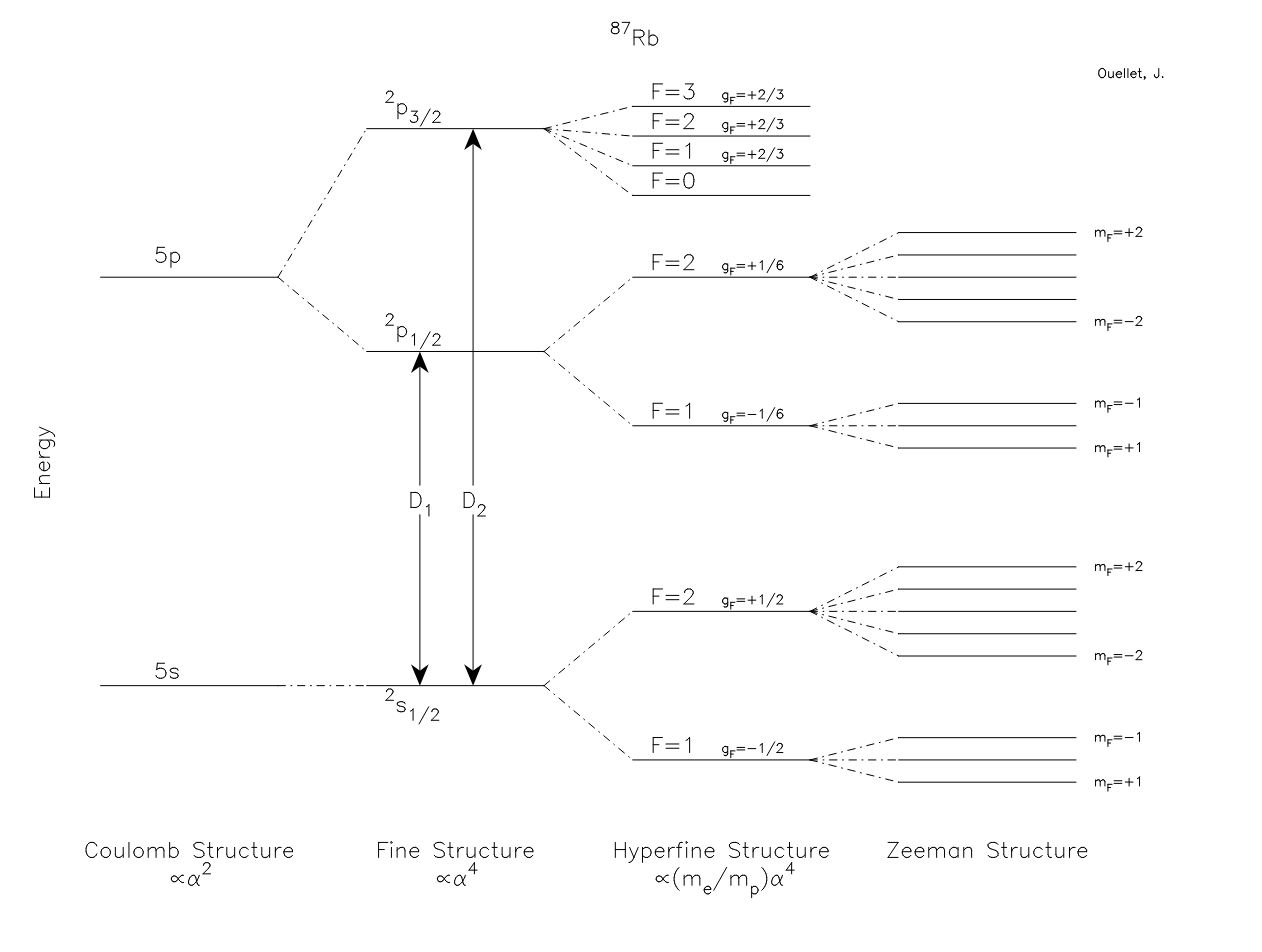
\includegraphics[scale=0.5]{images/zeeman.png}	
		\caption{Diagram showing the energy splitting due to the Zeeman effect,
		provided to us by \cite{ouelletEnergyLevelsRb2010}.} 
		\label{zeeman}
	\end{figure}

	\subsubsection{The Breit-Rabi Formula}
	The Breit-Rabi formula gives a relationship between the resonance frequency of an
	atom and its relationship between it and the external magnetic field applied \(
	\mathbf{B}_\text{ext} \). Written, it is expressed as:
	\begin{equation}
		\label{breit-rabi}
		\frac{\nu}{\mathbf{B}_\text{ext}} = \frac{2.799}{2I + 1} \
		\frac{\text{MHz}}{\text{G}}
	\end{equation}
	Here, \( \nu \) is the resonant frequency and \( I \) is the nuclear spin. The
	derivation for this equation is rather long and involves using ladder operators
	\( L_+ \) and \( L_- \), so we won't go into it in extreme detail here. For
	further information, see the appendix. 

	\subsection{Optical Pumping}
	With the perturbation theory out of the way, we now turn to the some theoretical
	aspects of the experiment that we should become familiar with. To begin, the
	objective for our experiment is to measure the transitions between two quantum
	states \( \ket*{F, m_F} \) and \( \ket*{F, m_F \pm 1} \) in an atom. However, the
	probability of an atom existing in either of these two states is actually equal,
	which we can see in the following equation:  
	\[
		\frac{P_2}{P_1} = \exp\left( - \frac{E_2 - E_1}{k_BT} \right)
	\]
	This is because the distribution of energies follows a Boltzmann distribution,
	and the states \( \ket*{F, m_F} \) and \( \ket*{F, m_F \pm 1} \) have the same
	energy. Thus, in order for us to see a transition, we need to alter this
	probability somehow. This is the method which we call \textit{optical pumping}.
	Optical pumping involves sending in polarized light, which changes this
	distribution by causing the electrons in the atom to excite, giving the
	transition \( \ket*{F, m_F} \to \ket*{F, m_F + 1} \). Then, the electron emits
	infrared light, and changes \( m_F \) by \( \Delta m_F = \{-1, 0, 1\} \)
	with equal probability. Because the excitation step only increases the quantum
	number, then over many iterations we will find that the value \( m_F \) 
	tends to increase, and thus we will eventually get all the atoms in the state 
	with the highest energy, which, in the case of a magnetic field in the \( z \)
	direction, corresponds to the highest possible \( m_F \). This is not true in
	general of course -- if the magnetic field direction were flipped, then the
	lowest value of \( m_F \) would be the highest energy state. This highest energy
	state is also called the \textit{pumped state}, which is the term I will be using
	to describe it in the rest of this report.  

	In the highest \( m_F \) state, the electrons cannot absorb any more light, since
	the absorption requires that we increase \( m_F \) by one. As a result, when the
	atoms reach this state, they become unable to absorb the polarized light, and are
	considered to be in a "dark" state. In order to bring them out of this state, we
	drive the atoms with a radio frequency (RF) magnetic field, which has the effect
	of driving the atoms out of the pumped state, into states which can absorb more
	light. We can detect such changes through the use of a photodetector positioned
	directly to measure the amount of light that passes through the atoms -- if the
	atom is not in the dark state, then the electrons will absorb the light we feed
	it and the photodetector will read a low light level, whereas in the dark state
	since no light is absorbed the photodetector will read a high light level. With
	this setup, we are now able to detect the required atomic transitions.

	\section{Experimental Setup}
	A diagram of the experimental setup used is shown in figure \ref{setup}.
	The main component of our experimental setup is the small glass bulb in the
	middle, which sits in an insulating metal box. This glass bulb contains our
	\ch{^{85}Rb} and \ch{^{87}Rb} atoms, along with an
	inert gas. At room temperature, the rubidium atoms exist as a solid which coats 
	the walls of the glass. This is not ideal, and instead we want some of the 
	rubidium atoms to exist as a gas, so to achieve this we heat the bulb to a
	temperature such that some of the rubidium atoms would be promoted to a gaseous
	state. This heating is achieved through a resistive heating element, controlled
	by the heating control unit. A thermometer is placed inside the insulating box to
	so we can monitor the temperature in the bulb, allowing us to keep the
	temperature approximately constant throughout the experiment.   

	\begin{figure}[h]
		\centering
		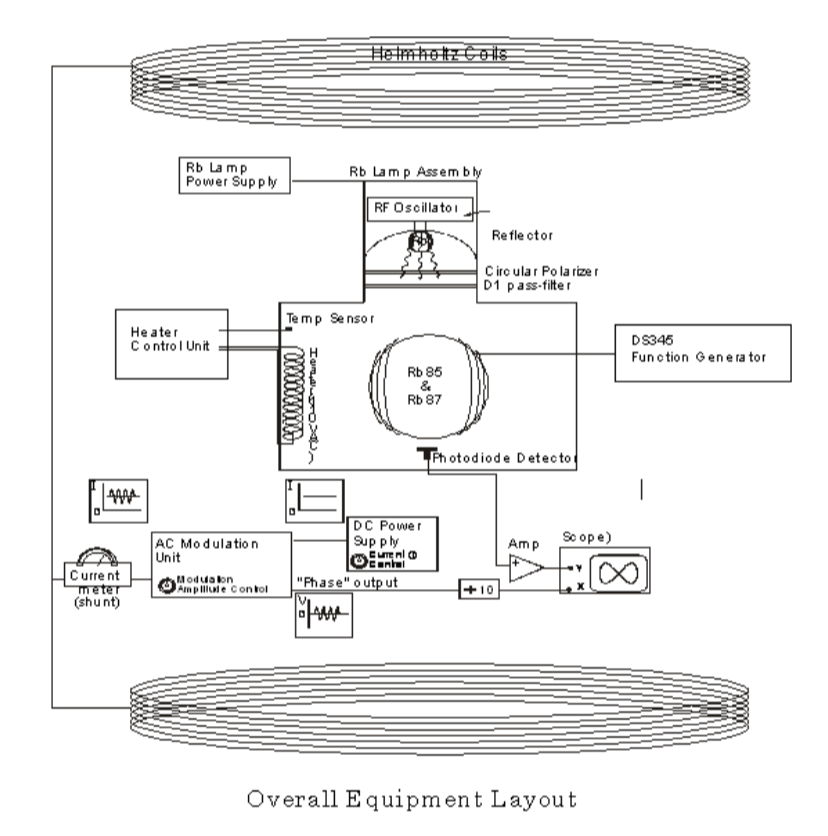
\includegraphics[scale=0.5]{images/setup.png}
		\caption{Block diagram of the experimental setup with labeled components,
		provided by \cite{lab-manual}.}
		\label{setup}
	\end{figure}

	Surrounding the bulb are two metal coils which connect to a DS345 function
	generator. These coils are responsible for generating the RF magnetic field that
	drives pumped atoms out of the aforementioned "dark state", back into a state
	where they can absorb polarized light. Next, we have a lamp assembly at the 
	top of the box, whose
	light is sent through a circular polarizer to keep only the circularly polarized
	portions of the light. The light that goes through the gas is then captured by
	the photodiode at the bottom of the box, after it passes through the rubidium
	gas. The signal from the photodiode also tends to be small (since only a small
	amount of rubidium atoms actually release into the gas), so we pass the signal
	through a signal amplifier before it is fed into the oscilloscope.          

	Finally, the last component of our experimental setup is are the large Helmholtz
	coils that surround the thermally insulating box. The coils are connected to an
	alternating current source, which is the source of our magnetic field \(
	\mathbf{B}_\text{ext} \) that generates the Zeeman effect. The coil has \( N =
	135 \) turns and a radius \( a = 27.5 \) cm, parameters that will become
	important when we calculate \( \mathbf{B}\text{ext} \). 
	The current is measured through a current meter (shunt), 
	which tells us the strength of the magnetic
	field we are using. The phase is also output through a separate channel; its use
	will be clear in the next section.  

	\section{Experimental Procedure}

	In this section, we detail the experimental procedures we carried out during this
	experiment. Due to the multitude of measurements we will be taking, this section
	will be broken down into subsections, under which the specific procedure for each 
	section is detailed. There are some common steps we took with each measurement,
	which we will detail in the following paragraph. 

	First, we would turn on all the relevant electronic devices (scopes, function
	generators, etc.), and begin by using the temperature controller to heat the
	the insulating box containing the rubidium to a temperature around \( 53^{\circ}
	\)C, then we would turn off the heating element, as it produces a magnetic field
	strong enough to interfere with our measurements. The heating element would
	remain off until the temperature got below \( 40^{\circ} \)C, after which we
	would restart the heater until the temperature rose \( 53^{\circ} \)C again.           
	Along with the procedure, some preliminary background calculations
	will be made; these are quantities that are not data but information given to us,
	so we will calculate them here. 

	\subsection{Observation of ODMR}

	The objective of this section is to experimentally confirm that the optical
	pumping procedure "works", as intended, and we can experimentally verify the
	presence of the Zeeman splitting and resonance. To do this, we will use the large
	Helmholtz coils, and pass a fixed DC current through it. When we pass a DC
	current through the coils, it generates a magnetic field, which due to the coil
	separation and overall geometry, can be approximated as a constant magnetic field
	-- that is, the vector \( \mathbf{B} \) field is a constant vector between the
	coils. With this approximation in hand, we can derive a formula for the strength
	of the magnetic field (this comes from basic electrodynamics):
	\begin{equation}\label{helmholtz}
		B = \frac{32 \pi N I}{5\sqrt{5}a} \times 10^{-7}\ \text{Tesla}
		= \frac{32 \pi N I}{5\sqrt{5}a} \times 10^{-3}\ \text{Gauss}
	\end{equation}
	For this section, we are instructed to keep the current at \( I = 1 \) A, so with
	\( N = 135 \) turns and \( a = 27.5 \) cm, we are able to conclude that the
	strength of the magnetic field at \( I = 1 \) A is:
	\[
		\mathbf{B}_\text{ext} = 4.41 \times 10^{-4} \ \text{T} = 4.41 \ \text{G}
	\]
	Recall that 1 Gauss = 1000 Tesla. Now, with this knowledge, we can calculate the
	resonant frequencies of \ch{^{85}Rb} and \ch{^{87}Rb} using the Breit-Rabi
	formula from earlier, substituting this value of \( \mathbf{B}_\text{ext} \) in.
	So, we get:
	\[
		\nu_{\text{Rb85}} \approx 2.059 \text{ MHz} \quad \nu_{\text{Rb87}} \approx
			3.087 \text{ MHz}
	\]
	% consider moving this to the later sections. 
	To verify these ODMR resonances, we first heat up the chamber, then set the DS345
	function generator to sweep over sine waves of a defined frequency range. The
	sweep also has an associated sweep period, a parameter which also needs to be
	carefully tuned to see the ODMR peaks. To see why, consider a sweep over the
	frequencies between 2-3 MHz. This covers both the resonance peaks calculated
	above, so we should see two peaks in the sweep. However, these peaks would only
	be present if there were atoms in the \( m_F = 0 \) state which had the ability
	to excite (recall that the atoms reside in the "dark state" until they are
	down pumped), meaning that if the sweep had been too fast, we would get fewer
	atoms in the \( m_F = 0 \) state, and as such this would lead to a shallower peak
	in the resonance measurement. While conducting the experiment, 
	we found that a sweep period of \( T = 1\)s worked out the best, but unfortunately 
	because it was so slow we couldn't
	really get a good picture of both peaks showing up on the oscilloscope. That
	said, we do confirm that we saw two resonance peaks, similar to those shown in
	figure \ref{ODMR}. 
	\begin{figure}
		\centering
		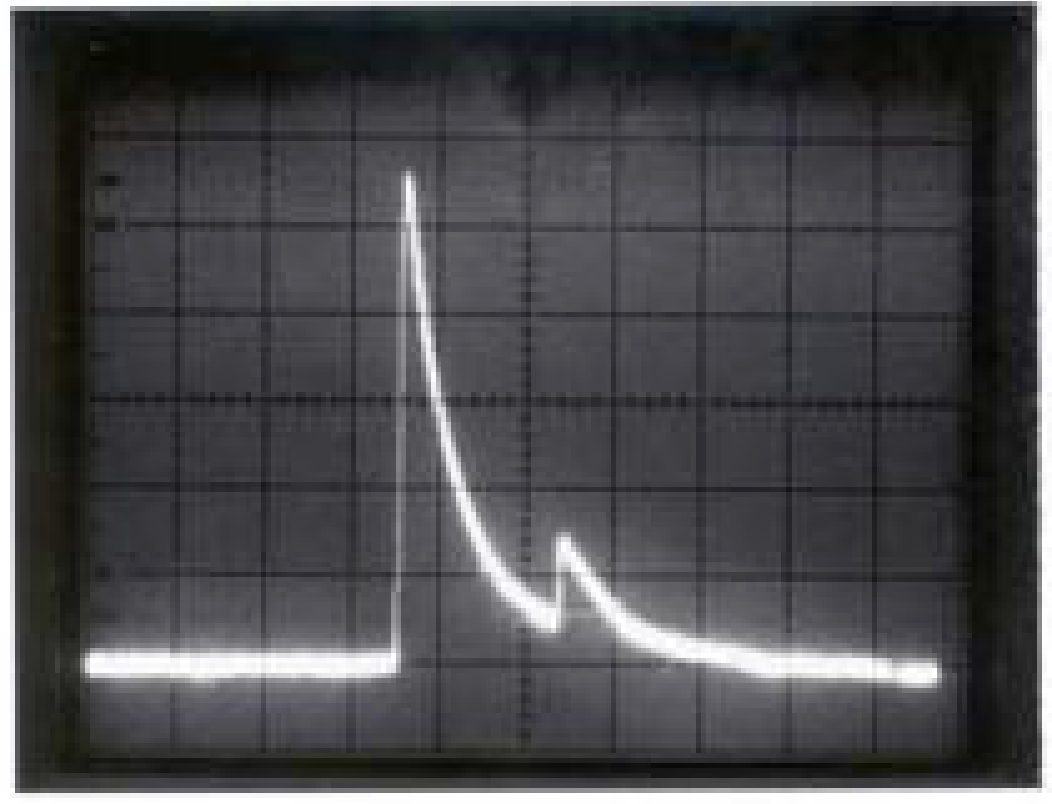
\includegraphics[scale=0.5]{images/ODMR.png}
		\caption{ODMR peaks on the oscilloscope when sweeping over an appropriate
			frequency range. This image was taken from \cite{lab-manual}, 
			because we could
		not get a good image showing the entire sweep range as an image.}   
		\label{ODMR}
	\end{figure}
	Finally, the last measurement we took in this step was to approximately determine
	the resonance frequencies of \ch{^{85}Rb} and \ch{^{87}Rb}. To do this, we
	gradually narrowed down the frequency sweep range so that the left edge of the sweep
	would be as close to the resonant frequency as possible; this was obviously
	repeated for both isotopes. These measurements were intentionally crude, mainly
	because more precise measurements would be made later in the lab anyway, so this
	measurement serves only as an approximate guide so we know in which frequency
	range we should expect to see each peak. From these
	measurements, we found that the resonances for \ch{^{85}Rb} and \ch{^{87}Rb} were
	approximately 1.9 MHz and 2.8 MHz, respectively. % check these numbers 

	\subsection{Good settings for bulb temperature}
	In this section, the objective was to determine the optimal temperature of the
	bulb for our measurements. That is, because the experimental apparatus is
	inherently temperature dependent, our objective was to find the ideal temperature
	for our measurements such that we see the maximum resonance. To do this, we first
	heat the chamber to around \( 52^{\circ} \)C, and continue to do the frequency
	sweep outlined in the previous section, with the sweep range narrowed down so
	that we see only one of the two peaks. This temperature was chosen because it was
	as close to \( 55^{\circ} \)C as we were comfortable in approaching, as the lab
	manual instructed us to not exceed this temperature. Then, as the temperature
	decreased over time, we recorded the temperature and also the amplitude of the
	resonant peak. This measurement was done by eye, by counting the height of the
	peak using the number of grid lines the peak passes through. We did this over a
	temperature range from approximately \( 42^{\circ} \)C to \( 52^{\circ} \)C, and
	the dependence on temperature we obtained is given in table
	\ref{bulb-temperature}, and a scatter plot of this relationship is shown in
	figure    
	\ref{resonance-vs-temperature}. For the errors in our measurements here, we are
	confident in counting the number of grid lines up to 0.3 of a grid\footnote{this
		is relatively generous, but it is much preferred to overestimate than to
	underestimate the error.}, which is also displayed on the plot.  

	\begin{figure}
		\begin{subfigure}{0.5\textwidth}
			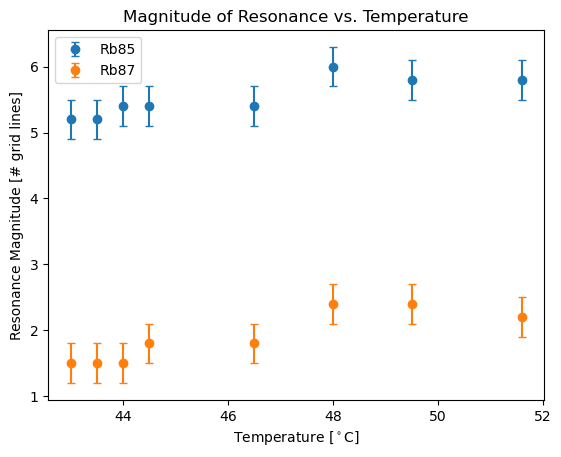
\includegraphics[scale=0.5]{images/resonance-vs-temperature.png}
			\caption{}
			\label{resonance-vs-temperature}
		\end{subfigure}
		\begin{subfigure}{0.5\textwidth}
			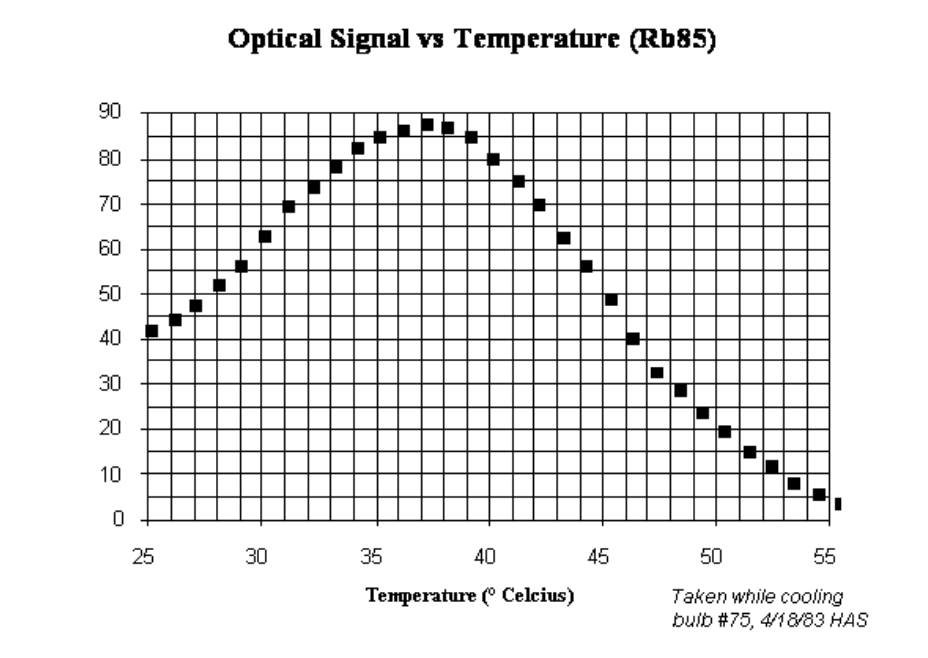
\includegraphics[scale=0.5]{images/resonance-vs-temperature-manual.png}
			\caption{}
			\label{resonance-vs-temperature-manual}
		\end{subfigure}
		\caption{(a) Measured resonance magnitude and its relationship to
			temperature. Note that while we do observe the peak resonance at
			approximately \( 48^{\circ} \)C, we do find that the variation across the
			entire temperature range is not significant enough for it to drastically
		impact our measurements. (b) A plot of the same experiment, provided to us by
		\cite{lab-manual}.}
	\end{figure}

	As is evident in the plot, we found that while there are small changes in the
	amplitude of the peak, the changes are not very significant over the span of the
	entire temperature range we took data in. While this does not replicate the plot
	that was given to us in \cite{lab-manual} (figure
	\ref{resonance-vs-temperature-manual}), this is not incredibly
	alarming however, because not only is figure
	\ref{resonance-vs-temperature-manual} a plot of an entirely
	different experiment, but these results really just tell us that any measurements
	between \( 42^{\circ} \)C to \( 51^{\circ} \)C should be significant enough 
	that they are detectable, and we don't need to be incredibly specific about the 
	temperature we take the data at. 

	That said, it would certainly have been nicer to demonstrate that the temperature
	range of approximately \( 40^{\circ} \)C to \( 50^{\circ} \)C was 
	an \textit{ideal} range
	to take our data in rather than an acceptable range, but this would require us to
	have taken more data below \( 40^{\circ} \)C, which we did not do. 

	\subsection{Lock-in detection of the Resonance Frequency} 
	\label{lock-in}

	For this section, the objective is to carry out a more precise measurement of the
	resonance frequency, as we outlined earlier how the approach of determining the
	resonance through sweeping was incredibly imprecise (not to mention also very
	tedious as well). Instead, a more precise method of determining the resonance
	frequency would be to find the current needed through Helmholtz coils to produce
	resonance, while holding the RF pumping at a specific frequency. The reason this
	is because the down-pumping step is very sensitive to frequency variations, so
	even if the down-pumping frequency were slightly off there would be very few
	atoms which successfully pump down. This provides us with far greater accuracy
	over our measurements than the sweep strategy we had earlier, for obvious
	reasons. 

	In addition to this, we also introduce a "lock-in" method for detection, which
	involves sending an AM modulated signal to the Helmholtz coils instead of DC.
	There are two main reasons we do this: firstly, the modulation allows us to send
	in an AC signal, which allows us to reduce the noise in the system, as there
	aren't many noise sources at high frequency when compared to low frequency.
	Second, this AC modulation also allows us to sweep over the Zeeman resonance
	many times per second in a single cycle of the envelope wave, effectively giving
	us more measurement data.\footnote{Even though this isn't data we directly
		collect, these extra passes through the data really help us in determining
	the resonance peaks.} Plotting the modulated current signal on the \( x \)-axis
	of the scope and the photodiode signal on the \( y \)-axis, we see what is called
	a \textit{Lissajous curve} on the scope screen, as shown in figure
	\ref{lissajous}.

	\begin{figure}
		\centering
		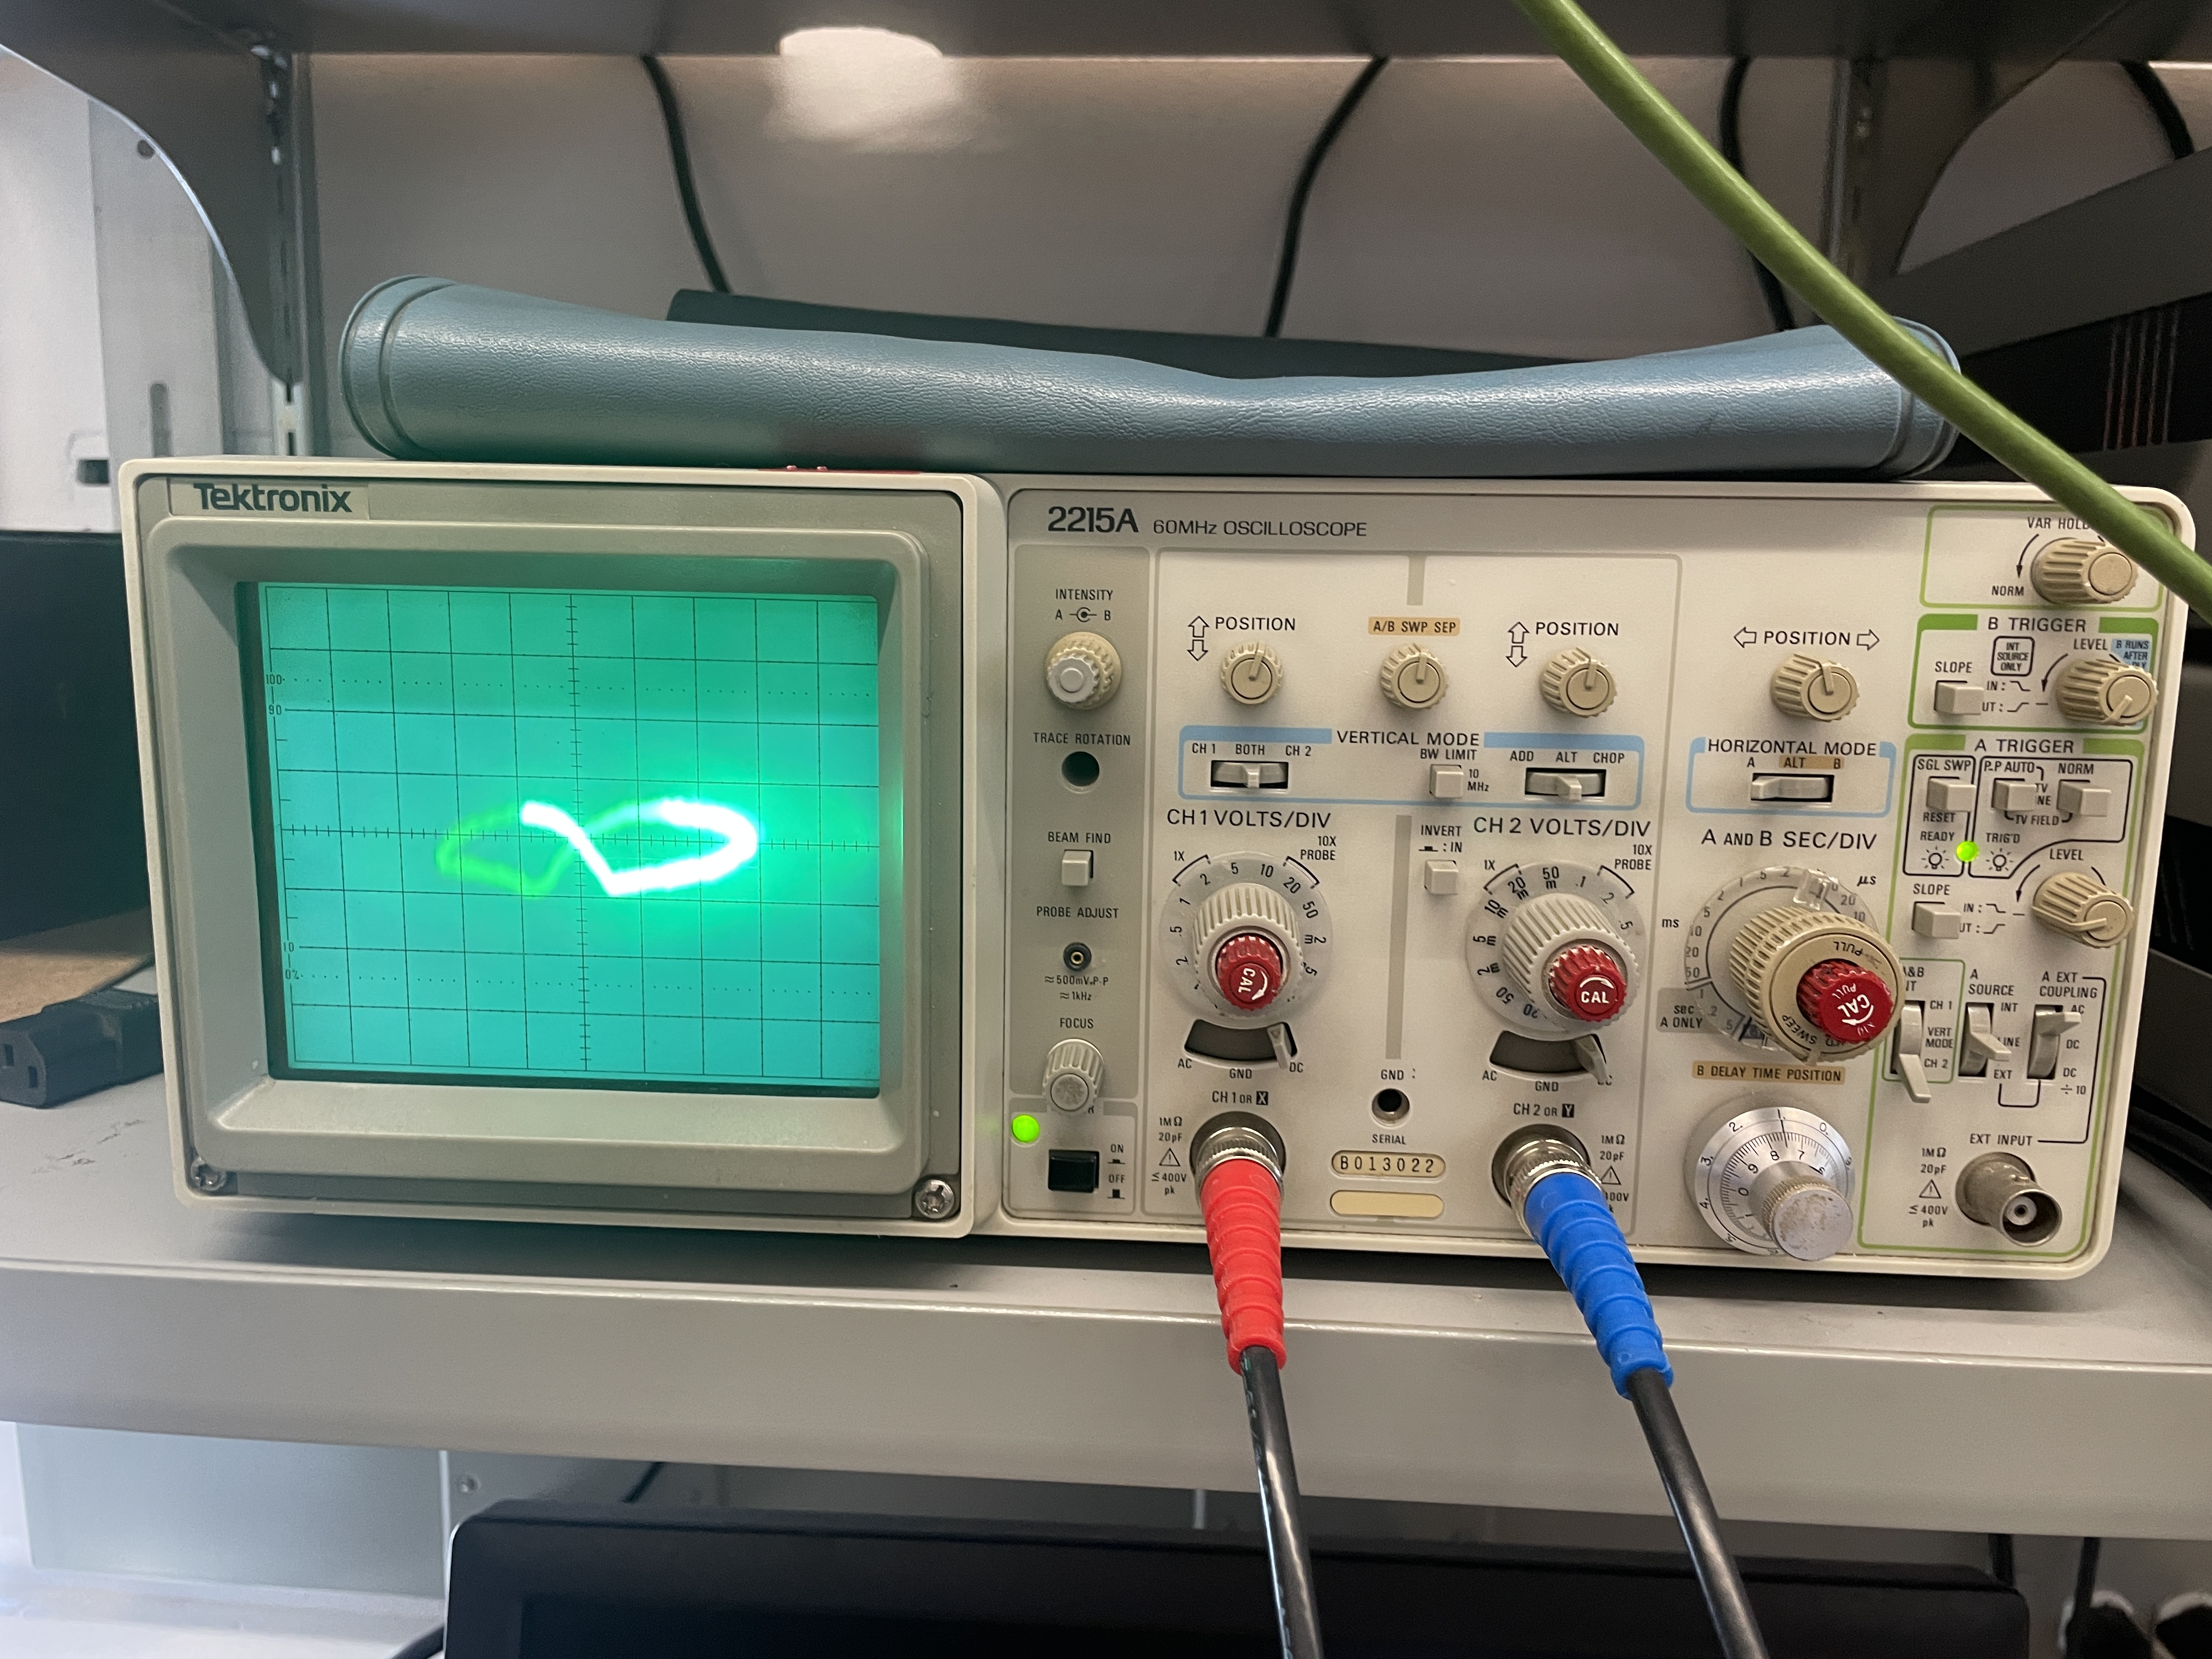
\includegraphics[scale=0.3]{images/lissajous.jpg}
		\caption{Centered Lissajous curve on the oscilloscope screen. On the \( x
			\)-axis is the modulated current signal, the \( y \)-axis is the
		photodiode signal. Note that the intersection of the Lissajous curve onto
	itself is exactly on the \( y \)-axis, which is what we define to be "centered".}
		\label{lissajous}
	\end{figure}
	
	At resonance, we should see an equal spike in the photodiode signal on both the
	positive and negative edge of the modulated current, due to symmetry. On the
	scope, this manifests itself as a \textit{symmetric} Lissajous curve along the \(
	y\)-axis. That is, the intersection of the Lissajous curve onto itself occurs on
	the vertical axis, which is exactly what is depicted in figure \ref{lissajous}.
	In order to capture such a shape, we first set the RF function generator to some
	frequency around the previously captured resonant frequency, then vary the
	modulated current until we observe a symmetric signal on the scope. Then, to
	determine the uncertainty bounds on our measurements, we continue varying the
	current, and record the current values at which the Lissajous curve becomes
	clearly asymmetric. In terms of the data we took, we captured data for 7 
	different RF frequencies,
	for both isotopes, and each RF frequency was captured twice: once for forward and
	reverse polarity, the latter of which was achieved by simply reversing the
	direction of the current. 

	\subsection{Zero-Field Resonance}

	In this section, we tune the Helmholtz coils to generate a magnetic field that
	exactly cancels Earth's magnetic field, placing the box in what is effectively a
	"zero field". Then, we vary the current exactly as before to find a symmetric
	Lissajous curve. The strength of the magnetic field is calculated using our
	measurements from the previous part.   

	\subsection{Timescale of Pumping} 
	In this section, the objective is to determine the characteristic time it takes
	for all the atoms to enter and leave the pumped state. To do this, we use the RF
	function generator to send a sinusoid signal modulated by a square envelope, and
	plot the photodiode signal over time. Then, we can record the signal on video,
	and determine the characteristic time by analysing the frames in the video. In
	order to maximize the accuracy of our measurement, this last step was done in a
	video editing software, in which it is possible to go through the video frame by
	frame. 

	\section{Analysis}

	\subsection{Resonance Frequency vs. Current} 
	The data we took for both isotopes is provided in table \ref{rb85} and table
	\ref{rb87}. The first portion of the analysis will be dedicated to experiment
	\ref{lock-in}, where the objective is to experimentally verify the Breit-Rabi
	formula (equation \ref{breit-rabi}). For convenience, the Breit-Rabi formula is
	reiterated below:
	\[
		\frac{\nu}{\mathbf{B}_\text{ext}} = \frac{2.799}{2I + 1} \
		\frac{\text{MHz}}{\text{G}}
	\]
	This \( \mathbf{B}_\text{ext} \) is the total magnetic field, so we need to split
	it into \( \mathbf{B}_\text{coil} + \mathbf{B}_\text{ambient} \), where \(
	\mathbf{B}_\text{coil} \) is the magnetic field generated by the large Helmholtz
	coils, and \( \mathbf{B}_\text{ambient} \) is the ambient magnetic field at
	Berkeley. Moving this \( \mathbf{B} \) term to the right hand side, we get the 
	following equation:
	\[
		\nu = \frac{2.799}{2I + 1}(\mathbf{B}_\text{coil} +
		\mathbf{B}_\text{ambient})
	\]
	In terms of the quantities we measure, we have resonant frequency \( \nu \) and
	also the magnetic field generated by the coil \( \mathbf{B}_\text{coil} \), so
	this equation suggests a linear fit between \( \nu \) and \(
	\mathbf{B}_\text{coil} \). The ambient magnetic field is dominated by Earth's
	magnetic field at Berkeley, which we can obtain from \cite{WorldMagneticModel2020} 
	to be \(
	\mathbf{B}_\text{ambient} = 47645.9 \) nT. One thing to note is that in our
	plots, we will be plotting the current on the \( y \)-axis, so in this case we
	actually need to rearrange this equation to solve for \( \mathbf{B}_\text{coil}
	\), which gives us the following equation:
	\begin{equation}
		\label{linear-fit}
		\mathbf{B}_\text{coil} = \frac{2I + 1}{2.799}\nu -
		\mathbf{B}_\text{ambient} 
	\end{equation}
	Then, substituting in the formula we have \( \mathbf{B}_\text{coil} \) in terms
	of the current, we will have our expected slope and \( y \)-intercept. This will
	be done later, after we have seen the plots. For now, we will move on to the
	scatter plot and the fits. 

	\begin{figure}
		\centering
		\begin{subfigure}{0.4\textwidth}
			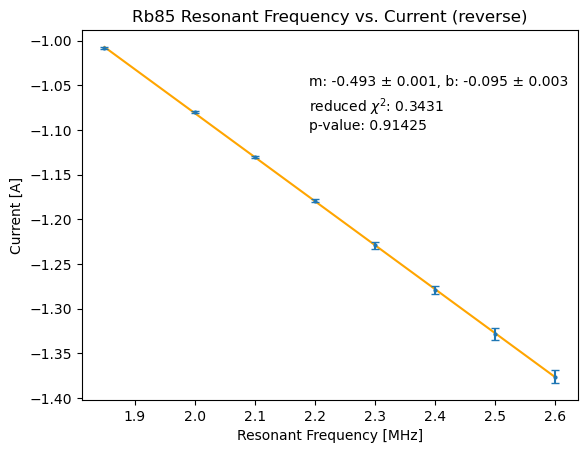
\includegraphics[scale=0.4]{images/rb85-neg.png}
			\caption{}
		\end{subfigure}
		\begin{subfigure}{0.4\textwidth}
			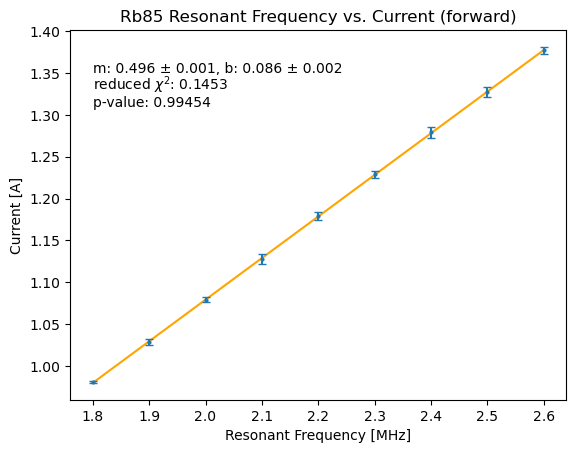
\includegraphics[scale=0.4]{images/rb85-pos.png}
			\caption{}
		\end{subfigure}
		\begin{subfigure}{0.4\textwidth}
			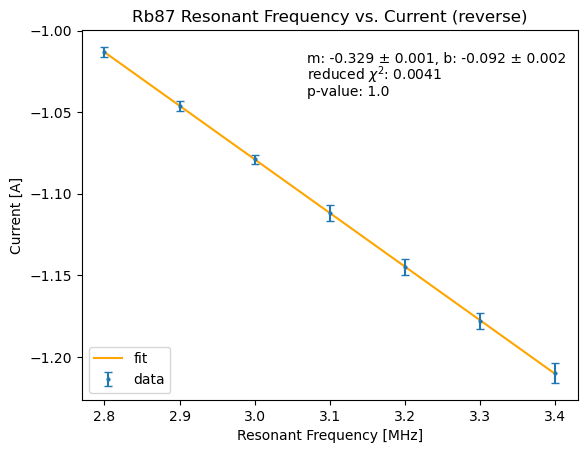
\includegraphics[scale=0.4]{images/rb87-neg.png}
			\caption{}
		\end{subfigure}
		\begin{subfigure}{0.4\textwidth}
			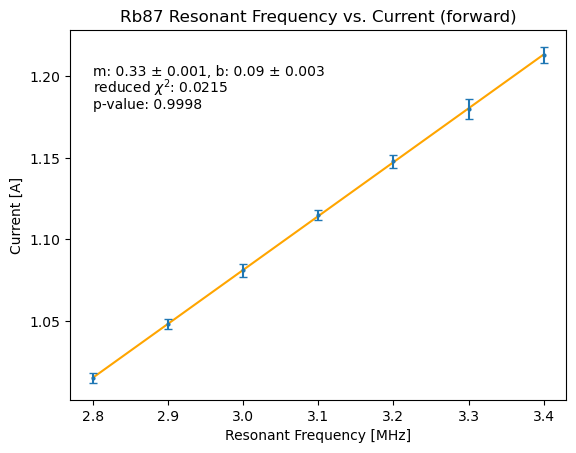
\includegraphics[scale=0.4]{images/rb87-pos.png}
			\caption{}
		\end{subfigure}
		\caption{Resonant frequency vs. Current for \ch{^{85}Rb} and \ch{^{87}Rb},
			for both forward and reverse polarities, computed using an unweighted
			linear fit. Statistical quantities such as \(
			\chi^2 \) and \( p \)-values are also calculated for each fit, and are
		displayed in their respective plots.}  
		\label{res-current}
	\end{figure}

	The scatterplot of the data and an unweighted least squares fit can be found in
	figure
	\ref{res-current}. As can be seen in the plots we fit the data to a linear
	function of \( y = mx + b \), and use \texttt{scipy.optimize.curve\_fit()} to
	perform a least-squares fit on the data. 
	As can be seen in the plots, the reduced \( \chi^2 \)
	values for all the plots are less than 2, which is considered a good fit
	according to \cite{hughesMeasurementsTheirUncertainties}. 
	Their associated \( p \)-values
	also suggest that our null hypothesis (in this case, the linear fit) is to be
	trusted, which confirms the linear relationship we expect as predicted by
	equation \ref{breit-rabi}. One additional plot we can generate using this data is
	to plot the positive and negative polarities together. To do this, all we have to
	do is flip the resonance frequencies for the polarities to a \textit{negative}
	frequency; physically a negative frequency doesn't really make much sense, 
	but one way to think about this is in the same way negative momentum is
	interpreted: as a wave moving in the opposite direction. 
	
	\begin{figure}
		\centering
		\begin{subfigure}{0.4\textwidth}
			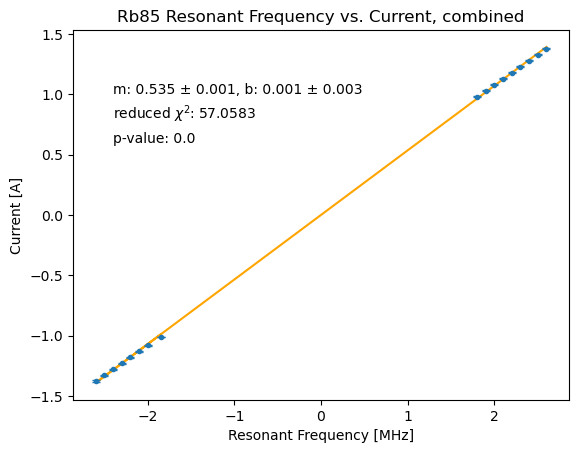
\includegraphics[scale=0.4]{images/rb85-combined.png}
			\caption{}
		\end{subfigure}
		\begin{subfigure}{0.4\textwidth}
			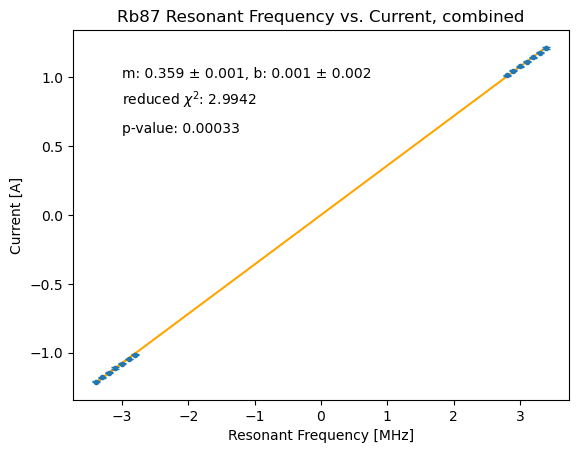
\includegraphics[scale=0.4]{images/rb87-combined.png}
			\caption{}
		\end{subfigure}
		\caption{Resonant frequency vs. Current for \ch{^{85}Rb} and \ch{^{87}Rb} for
			both current polarities combined,
			computed using an unweighted least-squares fit. 
			Statistical quantities such as \( \chi^2 \) and \( p \)-values are also 
		calculated for each fit.}  
		\label{res-current-combined}
	\end{figure}

	Figure
	\ref{res-current-combined} shows the least-squares fit when both polarities are
	combined.
	Unlike the individual plots, we find that the \( p
	\)-value of this plot is 0, which indicates to us that the errors in this plot
	are statistically significant enough that our null hypothesis (our linear fit) 
	should be rejected. In addition, the reduced \( \chi^2 \) values for both these
	plots are too large (\cite{hughesMeasurementsTheirUncertainties} gives \( \chi^2
	\geq 1.5 \) as the threshold) so this statistic also indicates that our fit is 
	not to be trusted.    
	This is to be expected, since it makes no sense to have a current associated with
	a resonance frequency when we set the function generator to output a DC signal;
	the down-pumping requires a signal whose frequency is equal to that of the energy
	gap from the Zeeman splitting, and such an energy is not achievable with a DC
	signal. As a result, we can't really determine the relationship around \( \nu = 0
	\).      

	With that said, the reason the \( p \)-values are so low is largely due to the
	extremely small uncertainties we have on our fitted values of \( m \) and \( b \)
	from the individual plots in figure \ref{res-current}. That is, taking a look at
	the \ch{^{85}Rb} individual plot, our values of \( m \) and \( b \) lie around \(
	m = 0.49 \pm 0.001, b = 0.09 \pm 0.002 \) (these values are intentionally crude;
	there's not much reason to be precise here, we'll see why in a moment), 
	whereas the fitted values for the
	combined plot in \ref{res-current-combined} is \( m = 0.535 \pm 0.001, b = 0.001
	\pm 0.003 \). Comparing the two values and their reported uncertainties, it's
	easy to see that they fall well outside of each other, up to many times the
	standard deviation. This would be the case even if we had been more precise with
	how we obtained a combined \( m \) and \( b \), since the uncertainties are just
	so small. As a result, the \( p \)-value for these two events
	simultaneously occurring is exceedingly low, which is why the combined plot gives
	us a \( p \)-value of zero.     

	\begin{figure}
		\centering
		\begin{subfigure}{0.4\textwidth}
			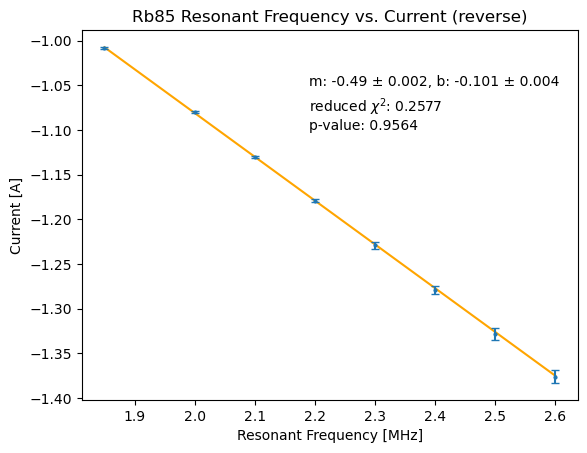
\includegraphics[scale=0.4]{images/rb85-neg-weighted.png}
			\caption{}
		\end{subfigure}
		\begin{subfigure}{0.4\textwidth}
			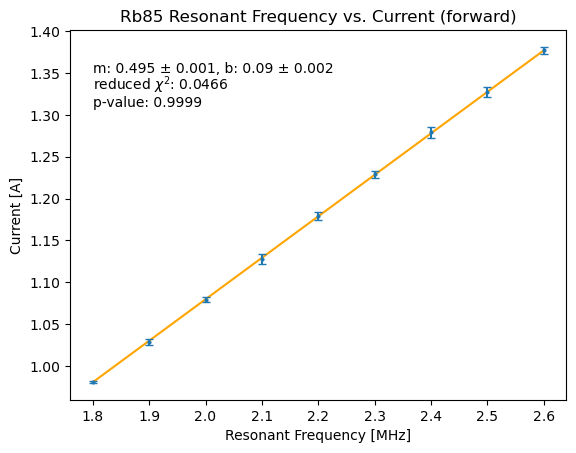
\includegraphics[scale=0.4]{images/rb85-pos-weighted.png}
			\caption{}
		\end{subfigure}
		\begin{subfigure}{0.4\textwidth}
			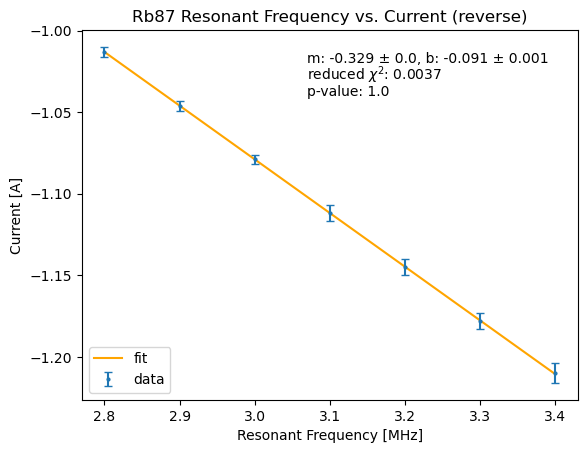
\includegraphics[scale=0.4]{images/rb87-neg-weighted.png}
			\caption{}
		\end{subfigure}
		\begin{subfigure}{0.4\textwidth}
			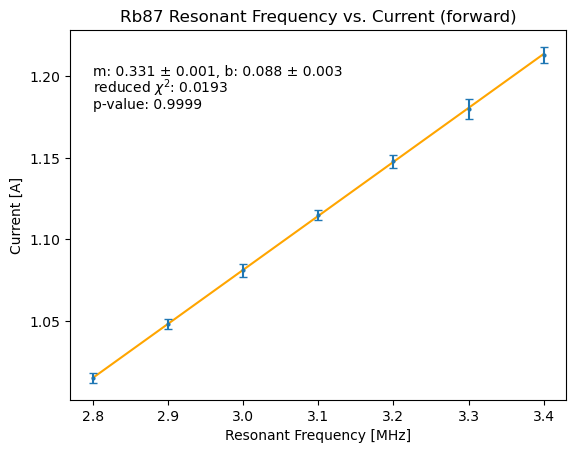
\includegraphics[scale=0.4]{images/rb87-pos-weighted.png}
			\caption{}
		\end{subfigure}
		\caption{Resonant frequency vs. Current for \ch{^{85}Rb} and \ch{^{87}Rb},
			for both forward and reverse polarities, computed using a weighted
			linear fit. Statistical quantities such as \(
			\chi^2 \) and \( p \)-values are also calculated for each fit, and are
		displayed in their respective plots.}  
		\label{res-current-weighted}
	\end{figure}
	\begin{figure}
		\centering
		\begin{subfigure}{0.4\textwidth}
			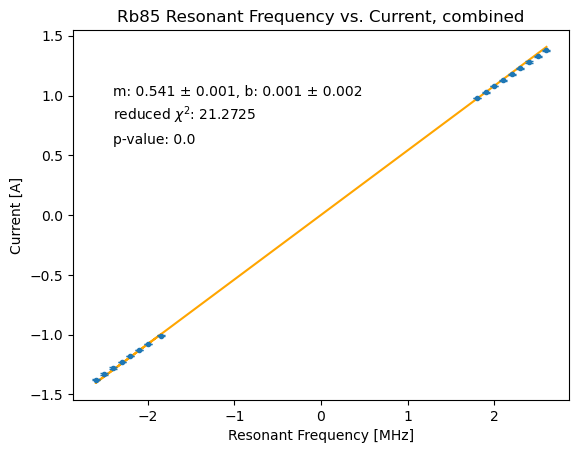
\includegraphics[scale=0.4]{images/rb85-combined-weighted.png}
			\caption{}
		\end{subfigure}
		\begin{subfigure}{0.4\textwidth}
			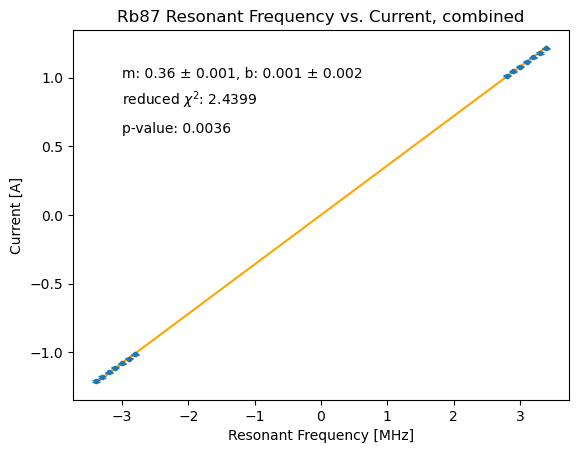
\includegraphics[scale=0.4]{images/rb87-combined-weighted.png}
			\caption{}
		\end{subfigure}
		\caption{Resonant frequency vs. Current for \ch{^{85}Rb} and \ch{^{87}Rb} for
			both current polarities combined,
			computed using a weighted least-squares fit. 
			Statistical quantities such as \( \chi^2 \) and \( p \)-values are also 
		calculated for each fit.}  
		\label{res-current-combined-weighted}
	\end{figure}

	In addition to an unweighted least-squares fit, we can also compute a weighted
	fit, using the same method we described in the EAX. Doing so, we obtain the plots
	shown in figures \ref{res-current-weighted} and
	\ref{res-current-combined-weighted}. Using the weighted fit, we can see that our
	\( p \)-values are much higher, the \( \chi^2 \) values are still below our
	threshold of \( \chi^2 \leq 2 \), which combine to again give us evidence that
	a linear fit is appropriate here. Despite incorporating the weights into our fit,
	this still doesn't really help our combined plots, which still have \( p
	\)-values near zero.  

	Comparing the fitted values of \( m, b \) between the weighted and unweighted
	fit, taking the negative polarity data \ch{^{85}Rb} as an example, we have the
	following:
	\begin{center}
		\begin{tabular}{c|cc}
				& unweighted      & weighted        \\ \hline
			\( m \) & \( -0.493 \pm 0.01\) & \( -0.49 \pm 0.002\) \\
			\( b \) & \( -0.095 \pm 0.03\) & \( -0.101\pm 0.004\)
		\end{tabular}
	\end{center}
	We can see that the weighted and unweighted fits agree relatively well. Thsi is
	to be expected, because based on our raw data, it is clear that there isn't any
	glaring outlier that we would like to weight less, which is precisely what a
	weighted least-squares fit attempts to mitigate against. Then, by this logic,
	every data point should be treated with equal weight, so therefore we will
	proceed with an unweighted least-squares fit for the rest of the analysis.   

	\subsection{Determination of Nuclear Spins}
	\subsubsection{Approach I}

	With the linear fits completed, the next thing we can determine is the nuclear
	spins of the rubidium atoms, which we can do by looking at the fit parameters. In
	particular, if we examine equation \ref{linear-fit} combine what we have from
	\ref{helmholtz}, we get the following relation:
	\begin{equation}
		\label{linear-fit-expanded}
		i = \frac{5\sqrt{5}a}{32 \pi N} \cdot 10^{3} \left( \frac{2I + 1}{2.799}\nu +
		\mathbf{B}_\text{ambient}\right) = \frac{1}{\alpha}\left( \frac{2I +
		1}{2.799}\nu - \mathbf{B}_\text{ambient} \right)
	\end{equation}
	where \( i \) is the current, and \( \alpha = \frac{32 \pi N}{5\sqrt{5}a} \cdot
	10^{3} \). 
	From this, we can extract the slope by looking at
	the prefactor of \( \nu \), and then ultimately solving for \( I \): 
	\[
		m = \frac{1}{\alpha} \frac{2I + 1}{2.799} \implies I = \frac{\alpha m \cdot
		2.799 - 1}{2}
	\]
	here \( m \) is the slope of the fit. The associated error is then given by:
	\begin{equation}
		\label{error-I}
		\delta_I = \sqrt{\delta_{\alpha}^2 \left( \frac{2.799m}{2}\right)^2 
			+ \delta_m^2\left( \frac{2.799 \alpha}{2}\right)^2}
	\end{equation}
	However, in our case, we claim that \( \delta_{\alpha} \) is actually zero,
	because there is no uncertainty in \( N \) (obviously), and there isn't any
	uncertainty reported in \( a = 27.5 \) cm, so we will treat it as an exact value,
	Thus, only the \( \delta_m \) term survives.  
	For our experimental value of \( m \), we will take the arithmetic mean
	of both current polarities for each isotope. If \( m_1, m_2 \) are the positive
	and negative polarity slopes and \( \delta_{m_1}, \delta_{m_2} \) are their
	respective uncertainties, then we know that the errors add in quadrature:
	\[
		\delta_{\overline m} = \sqrt{\delta_{m_1}^2\left( \frac{1}{2} \right)^2 +
		\delta_{m_2}^2\left( \frac{1}{2} \right)^2}
	\]
	So, this leaves us with the following slopes:
	\[
		\overline m_\text{Rb85} = 0.494 \pm 0.0079 \quad 
		\overline m_\text{Rb87} = 0.329 \pm 0.00059
	\]
	Note that the numbers are rounded in the report for simplicity, but they are kept
	exact during all calculations. Using these reported average slopes and their
	uncertainties, putting them into equation \ref{error-I}, we get:
	\[
		I_\text{Rb85} = 2.5557 \pm 0.0048 \quad
		I_\text{Rb87} = 1.5363 \pm 0.0036
	\]
	These values are incredibly close to the accepted values for nuclear spin, \(
	I_\text{Rb85} = 5 / 2 \) and \( I_\text{Rb87} = 3 / 2 \). This confirmation
	between the experimental and the theoretical values for the nuclear spin shows
	strong evidence that we are observing the exact phenomena we were looking for --
	the electron transitions between different Zeeman levels. 

	\subsubsection{Approach II}
	\label{approach-2}
	An alternative approach we can use to determine nuclear spins is to examine the
	ratios of the resonant frequencies for \ch{^{85}Rb} and \ch{^{87}Rb}. To do this,
	we return to the original Breit-Rabi formula from equation \ref{breit-rabi}:
	\[
		\frac{\nu}{\mathbf{B}_\text{ext}} = \frac{2.799}{2I + 1}
	\]
	Now, if we measure \( \nu \) for each isotope at the same intensity of \(
	\mathbf{B}_\text{ext} \), then we can divide the two together to get a ratio of
	the resonant frequencies for the same magnetic field strength:
	\[
		\frac{\nu_{85}}{\nu_{87}} = \frac{2 I_{87} + 1}{2 I_{85} + 1} = \frac{2}{3}
	\]
	In this equation, because we did not record any uncertainties for our frequency
	values, we unfortunately won't be able to perform error propagation on this
	equation. Further, because we controlled the current instead of the resonant
	frequency, we cannot guarantee that we have the same strength of \(
	\mathbf{B}_\text{ext} \) for any of the data points; to remedy this, we will
	instead make use of the average linear fits we obtained in the previous section 
	to get the resonant frequencies for a given current value for both isotopes. The
	errors in these values we can then propagate to find an "average error" of the
	resonance frequency ratio. 

	To be a more specific in how we computed this value, we first chose a common
	range of currents, and sampled 20 points within this range. Then, from our linear
	fit, we used the following equations to calculate the corresponding resonance
	frequency and its error:
	\[
		x = \frac{-b + y}{m}, \quad \delta_x = \sqrt{\delta_b^2 \left( -\frac{1}{m}
		\right)^2 + \delta_m^2 \left( \frac{b - y}{m} \right)^2}
	\]
	We repeat this for both the \ch{^{85}Rb} and \ch{^{87}Rb} samples, and then
	compute the ratio and its corresponding error:
	\[
		\text{ratio} = \frac{\nu_{85}}{\nu_{87}}, \quad 
		\delta_\text{ratio} = \sqrt{\delta_{85}^2 \left( \frac{1}{\nu_{87}} \right)^2
		+ \delta_{87}^2 \left( - \frac{\nu_{85}}{\nu_{87}} \right)^2}
	\]
	then as a final step, we take the average of both the ratio and its uncertainty
	to generate a final report for our experimentally calculated nuclear spin ratio.
	Doing so for the positive and negative polarities separately, we get ratios of
	\( 0.66659 \pm 0.032 \) for the positive and \( 0.66624 \pm 0.030 \) for the
	negative polarity. These two values both agree very well with the predicted value
	of \( \frac{2}{3} = 0.\overline 6 \), so this calculation gives us further
	agreement between the data and our theory, and also verifies that our previous
	calculations for \( I_{85} \) and \( I_{87} \) agree well with our theory.
	
	\subsection{Accuracy of Helmholtz Coils}

	The next thing we are asked to determine is to take a look at the accuracy of the
	Helmholtz coils, by picking a value of positive and negative polarity, and use
	our determined value for the nuclear spins to solve for the strength of \(
	\mathbf{B}\). We use the same coil for \ch{^{85}Rb} and \ch{^{87}Rb}, so picking
	one positive and negative current is enough -- no need to pick two separately for
	the two isotopes. So, we choose the resonance at \( \nu = 1.85 \) MHz for the
	negative polarity and \( \nu = 1.8 \) MHz for the positive. Using 
	equation \ref{linear-fit}, we get:\footnote{I am still doing the error
		propagaion, but I do feel like I've written it out enough times that it's
	clear I know how to do it; from here on out I won't keep writing it.}
	\[
		\mathbf{B}_\text{coil, negative} = 3.563 \pm 0.059 \text{ G}\quad 
		\mathbf{B}_{\text{coil, positive}} = 3.454 \pm 0.059 \text{ G}
	\]
	Calculating this using equation \ref{helmholtz} using the measured current, we
	get:
	\[
		\mathbf{B}_\text{coil, negative} = 4.44 \pm 0.021 \text{ G}\quad
		\mathbf{B}_\text{coil, positive} = 4.33 \pm 0.021 \text{ G}
	\]
	we can see that the predicted magnetic field strength is vastly different than
	what we should theoretically be getting from the Helmholtz coils. This difference
	is more than statistically significant, but at the same time this is to be
	expected, especially considering that the equipment in this lab is at least twice
	my age. Furthermore, there are also other sources of error, such as our limited
	accuracy on the Bohr magneton \( \mu_B \), though this source of error, while
	existent, is not very likely to be the source of this discrepancy because the gap
	is simply too large for a better \( \mu_B \) to dramatically improve the
	agreement. 

	\subsection{Ambient Magnetic Field}
	Finally, the last thing we can calculate using this data is the ambient magnetic
	field strength. This quantity is contained in the \( y \)-intercept of the data,
	since according to equation \ref{linear-fit-expanded}, we have
	\[
		b = \frac{\mathbf{B}_\text{ambient}}{\alpha}
	\]
	We also computed an average \( y \)-intercept which we calculated in section
	\ref{approach-2}, so we can just use that value to determine \(
	\mathbf{B}_\text{ambient} \). Using this, we get:
	\[
		\mathbf{B}_\text{ambient, Rb85} = 0.401 \pm 0.0078 \text{ G}\quad 
		\mathbf{B}_\text{ambient, Rb87} = 0.402 \pm 0.0080 \text{ G}
	\]
	Compared to the ambient magnetic field at Berkeley given by
	\cite{WorldMagneticModel2020} of \(
	\mathbf{B}_\text{ambient} = 0.476459 \) G, this is relatively close, but our
	uncertainties are still too small to conclude that our calculated ambient
	magnetic field strength matches third-party data. Some possible sources for this
	discrepancy could be also due to the discrepancy in the strength of the Helmholtz
	coils -- after all, the discrepancy in the coil strength is a large systematic
	error, the absence of which could very well lead 
	to a better calculation of \( \mathbf{B}_\text{ambient} \). That said, with all
	things considered this value is still close enough that personally, I'd call this
	a relative success. 

	\subsection{Zero Field Measurement}
	The only unfortunate thing about our lab report is that we could not get the
	zero-field resonance to work properly. We aren't particularly sure what was the
	cause of this issue either; we did ask for assistance and none of the GSIs who
	helped us (including the professor) could figure it out. In principle, we could
	find the current required -- this would just be our \( y \)-intercept, 
	since it's the
	current value which corresponds to a resonant frequency of 0, or in other words
	the point when the degeneracy in the Zeeman levels is restored, indicative of
	zero field. 
	Therefore, we can just report our average \( b \)-value we got from the
	previous section as our current: \( i = 0.09 \pm 0.001 \) A. However, we have
	nothing to experimentally check this against, because we failed to collect the
	requisite data for this section. That said, we did hear from the GSIs that the
	value for this current should be very small so there is a chance this value is
	possibly close to the experimental value, but there's just no way for us to know.    

	\subsection{Characteristic Pumping Time}
	The final to analyze is the characteristic time for the pumping and de-pumping
	steps. To do this, we took a video of the photodiode signal over time while
	sending in a square modulated wave, and count the amount of time elapsed between
	the jumps. This process was completed using video editing software for the
	maximum accuracy (see figure \ref{video-editor}). That said, we still won't have
	errors in the traditional sense, because the video editing software (Adobe
	Premiere Pro) counts the number of frames as a discrete number, so there is no
	uncertainty. The data from this counting is given in table 
	table \ref{characteristic-time}, and computing the mean and standard deviation,
	we get:\footnote{We have to convert the frame data into seconds. The video was
	shot at 30 fps, so we can extrapolate the time duration of each from there.}   
	\begin{align*}
		t_\text{Rb85, up} &= 0.113 \pm 0.0053 \text{ s} & t_\text{Rb87, up} &= 0.113
		\pm 0.010 \text{ s} \\ 
		t_\text{Rb85, down} &= 0.125 \pm 0.013 \text{ s} & t_\text{Rb87, down} &=
		0.113 \pm 0.0053 \text{ s} 
	\end{align*}
	Due to the limited number of data points we took in this section, it's hard to be
	extremely confident in these statistics, but one good check here is that the two
	isotopes have the same characteristic time, which we do expect. The time it takes
	to pump the gas is also very close to the time it takes to de-pump, and this
	correspondence also gives credibility to our data, as this is also a phenomenon
	we expect. Overall, despite having more data points to sample, we do find that
	the data is consistent with our theory.  

	\begin{figure}
		\centering
		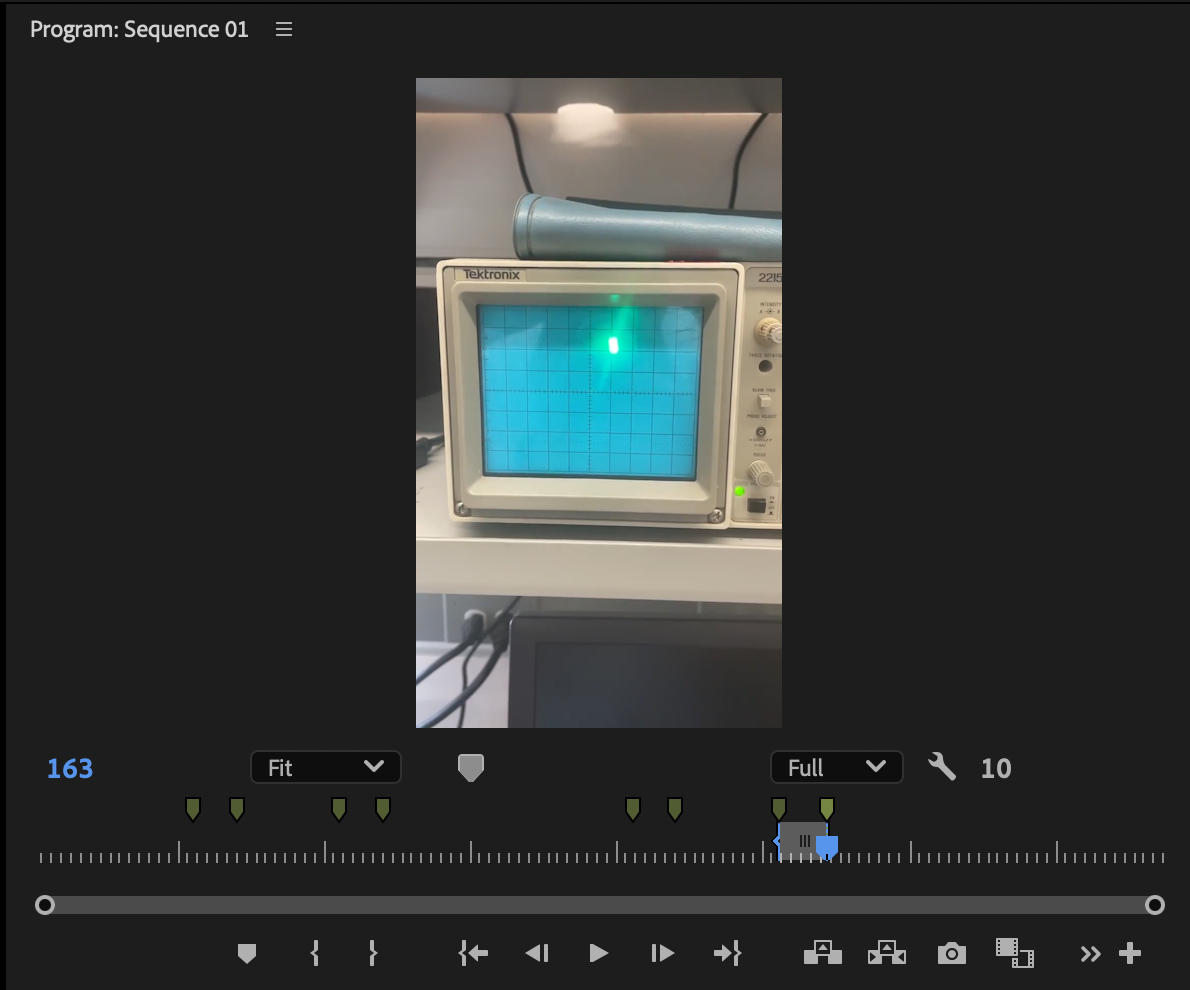
\includegraphics[scale=0.5]{images/video-editor.png}
		\caption{Screenshot of Adobe Premiere Pro, the software which was used to
			determine the characteristic time. This screenshot was taken when
			measuring the pumping time for \ch{^{85}Rb}; the green markers show the
			start and end of the pumping and the gray patch on the rail shows the
			window during which the sample is being pumped. The gray number on the
			right denotes how many frames have elapsed.}  
			\label{video-editor}
	\end{figure}	

	\section{Reflection \& Conclusion}

	Overall, our experimental data. and the results derived from them matched our
	expected theoretical results very well. We found a good correspondence between
	our linear fits and the data, both visually and also by comparing the slope and
	\( y \)-intercept to what we expect them to be numerically. We further confirmed
	the linear relationship we expect by experimentally calculating the individual
	nuclear spins for \ch{^{85}Rb} and \ch{^{87}Rb} in two different ways. In both
	methods, we get a remarkably good agreement between the experimental and
	theoretical values, which is strong evidence to support the fact that we are
	observing the expected Zeeman transitions.

	We then also calculated the ambient magnetic field, and comparing it to the
	ambient magnetic field at Berkeley, provided to us by
	\cite{WorldMagneticModel2020}, we find a
	relatively good agreement there as well (despite them not agreeing fully).  

	Our experiment isn't all full of successes, however. One major issue we ran into,
	and manifested itself as the lack of data for the zero field measurement, is the
	fact that we did not fully understand what we were doing before doing it. As a
	result, we spent \textit{way} more time on certain sections than we really should
	have, and this resulted in us not having enough time to fully work out the zero
	field measurement. This is also manifested in the resonance vs. current data,
	since there are some frequency values where we only have the current data for one 
	of the two polarities -- we initially did not establish a standard for which
	frequencies we would be using, and also did not have time at the end to go back
	and collect more data. Luckily, this did not affect our results very much, but
	there is easily a world where this does impact our experiment greatly and we walk
	away without good data to analyze. 
	Overall, this experiment was very fun and interactive: being able to tune the
	current until we see the effects of phenomena that we predicted
	all the way back in 137B (I took this a year and a half ago now) is
	incredibly satisfying, and shows that quantum mechanics does work!   

	% remember to talk about systematic errors in the reflection section 

	\nocite{*}
	\printbibliography

	\pagebreak
	\appendix
	\section{Raw Data}

	\subsection{Finding good settings for Bulb temperature} 

	\begin{table}[h!]
		\centering
		\begin{tabular}{|c|cc|}
			\hline
			\multirow{2}{*}{Temperature (\( \pm 0.1 \))} 
			& \multicolumn{2}{c|}{Resonant Frequency} \\
			\cline{2-3} 
										 & \multicolumn{1}{c|}{Rb85 (\( \pm 0.3 \))} &
										 Rb87 (\( \pm 0.3 \)) \\ \hline
			51.6 & \multicolumn{1}{c|}{5.8} & 2.2 \\
			49.5 & \multicolumn{1}{c|}{5.8} & 2.4 \\
			48.0 & \multicolumn{1}{c|}{6.0} & 2.4 \\
			46.5 & \multicolumn{1}{c|}{5.4} & 1.8 \\
			44.5 & \multicolumn{1}{c|}{5.4} & 1.8 \\
			44.0 & \multicolumn{1}{c|}{5.4} & 1.5 \\
			43.5 & \multicolumn{1}{c|}{5.2} & 1.5 \\
			43.0 & \multicolumn{1}{c|}{5.2} & 1.5 \\ \hline
		\end{tabular}
		\caption{Temperature vs. Amplitude of resonance. The uncertainty in our data
			is the same for all data points, so the uncertainty is listed at the top of
		the table.   }
		\label{bulb-temperature}
	\end{table} 

	\pagebreak
	\subsection{Resonance Frequency vs. Current}

	\begin{figure}[h!]
		\begin{subfigure}{0.5\textwidth}
			\centering
\resizebox{\columnwidth}{!}{%
\begin{tabular}{|c|cc|}
\hline
\multirow{2}{*}{Resonance Frequency (MHz)} & \multicolumn{2}{c|}{Current (A)} \\ \cline{2-3} 
 & \multicolumn{1}{c|}{Forward Polarity} & Reverse Polarity \\ \hline
1.8 & \multicolumn{1}{c|}{} & $-1.008 \pm 0.001$ \\
1.85 & \multicolumn{1}{c|}{$0.981 \pm 0.001$} &  \\
1.9 & \multicolumn{1}{c|}{$1.029 \pm 0.004$} &  \\
2 & \multicolumn{1}{c|}{$1.079 \pm 0.003$} & $-1.08 \pm 0.001$ \\
2.1 & \multicolumn{1}{c|}{$1.128 \pm 0.006$} & $-1.130 \pm 0.001$ \\
2.2 & \multicolumn{1}{c|}{$1.179 \pm 0.005$} & $-1.179 \pm 0.002$ \\
2.3 & \multicolumn{1}{c|}{$1.229 \pm 0.004$} & $-1.229 \pm 0.004$ \\
2.4 & \multicolumn{1}{c|}{$1.279 \pm 0.007$} & $-1.279 \pm 0.005$ \\
2.5 & \multicolumn{1}{c|}{$1.327 \pm 0.006$} & $-1.328 \pm 0.007$ \\
2.6 & \multicolumn{1}{c|}{$1.377 \pm 0.004$} & $-1.376 \pm 0.007$ \\ \hline
\end{tabular}%
}
\caption{}
\label{rb85}
		\end{subfigure}
		\begin{subfigure}{0.5\textwidth}
			\centering
\resizebox{\columnwidth}{!}{%
\begin{tabular}{|c|cc|}
\hline
\multirow{2}{*}{Resonance Frequency (MHz)} & \multicolumn{2}{c|}{Current (A)} \\ \cline{2-3} 
 & \multicolumn{1}{c|}{Forward Polarity} & Reverse Polarity \\ \hline
2.8 & \multicolumn{1}{c|}{$1.015 \pm 0.003$} & $1.013 \pm 0.003$ \\
2.9 & \multicolumn{1}{c|}{$1.048 \pm 0.003$} & $1.046 \pm 0.003$ \\
3.0 & \multicolumn{1}{c|}{$1.081 \pm 0.004$} & $1.079 \pm 0.003$ \\
3.1 & \multicolumn{1}{c|}{$1.115 \pm 0.003$} & $1.112 \pm 0.005$ \\
3.2 & \multicolumn{1}{c|}{$1.148 \pm 0.004$} & $1.145 \pm 0.005$ \\
3.3 & \multicolumn{1}{c|}{$1.180 \pm 0.006$} & $1.178 \pm 0.005$ \\
3.4 & \multicolumn{1}{c|}{$1.213 \pm 0.005$} & $1.210 \pm 0.006$ \\ \hline
\end{tabular}%
}
\caption{}
\label{rb87}
		\end{subfigure}
		\caption{Resonant Frequency vs. Current for both (a) \ch{^{85}Rb} and
			(b) \ch{^{87}Rb}. Note that while taking data for the \ch{^{85}Rb} dataset, 
			we made a mistake and took the current for \( \nu = 1.8 \) MHz for 
			reverse polarity only, and we took \( \nu = 1.9 \) MHz for the forward 
		polarity only.}
	\end{figure}
	\pagebreak
	\subsection{Characteristic Time} 
	\begin{table}[h!]
		\centering
\begin{tabular}{|cc|cc|}
\hline
\multicolumn{2}{|c|}{Rb85} & \multicolumn{2}{c|}{Rb87} \\ \hline
\multicolumn{1}{|c|}{$t_{\text{up}}$} & $t_{\text{down}}$ & \multicolumn{1}{c|}{$t_{\text{up}}$} & $t_{\text{down}}$ \\ \hline
\multicolumn{1}{|c|}{9} & 12 & \multicolumn{1}{c|}{10} & 10 \\
\multicolumn{1}{|c|}{9} & 10 & \multicolumn{1}{c|}{8} & 10 \\
\multicolumn{1}{|c|}{9} & 10 & \multicolumn{1}{c|}{10} & 10 \\
\multicolumn{1}{|c|}{10} & 9 & \multicolumn{1}{c|}{9} & 9 \\ \hline
\end{tabular}%
\caption{Characteristic time for the non-pumped gas to become pumped (\( t_\text{up}
\)) and the down-pumping time (\( t_\text{down} \)) for both isotopes. This number is
reported in frames, which is an exact quantity, so for that reason there are no
uncertainties.}
\label{characteristic-time}
	\end{table}
\end{document}

